\documentclass[10pt, xcolor=x11names]{beamer}
\usecolortheme{seagull}
\useoutertheme{infolines}
\usefonttheme[onlymath]{serif}
\setbeamertemplate{headline}[default]
\setbeamertemplate{navigation symbols}{}
\mode<beamer>{\setbeamertemplate{blocks}[rounded][shadow=true]}
\setbeamercovered{transparent}
\setbeamercolor{block body example}{fg=blue, bg=black!20}

\usepackage[utf8]{inputenc}
\usepackage[german]{babel}
\usepackage[]{csquotes}
\usepackage{amsmath}
\usepackage{tikz, wasysym}
\usepackage{graphicx}
\usetikzlibrary{automata,positioning}
\usepackage{hyperref}

%\usepackage{amsfonts}
%\usepackage{amssymb}
%\usepackage{makeidx}
%\usepackage{graphicx}


\usepackage{hyperref}
\author{Sven Fiergolla}
\title[Großes Studienprojekt]{Index Creation}
\subtitle[short version]{}
\date{\today}
%\institute[Uni Trier]{Universität Trier}
%\logo{\includegraphics[scale=.25]{unilogo.pdf}}

\begin{document}
	\frame{\maketitle}
	\frame{\frametitle{Übersicht}
	\tableofcontents
	}
	

	\section{Einführung}
	\frame{\frametitle{Einführung}

	Effiziente Suche über:
	\bigskip
	\pause\begin{description}
	\item Sammlung von Büchern
	\item das Web
	\item Große Datenmengen
\end{description}
\bigskip
\pause zu viel für Main Memory!

	}	
	
	\frame{\frametitle{Einführung}
Typische Systemeigenschaften (stand 2018)
\medskip
\begin{itemize}
	\item \textit{clock rate} 2-4 GHz, 4-8 Kerne
	\item \textit{main memory} 4-32 GHz
	\item \textit{disk space} $\leq$ 1 TB SSD oder $\geq$ 1 TB HDD
	\pause 
	\begin{itemize}
	\item HDD (hard disk drive)
	\begin{itemize}
	\item \textit{average seek time} zwischen 2 und 20 ms
	\item \textit{transfer time} 150 - 300 MB/s
	\end{itemize}
	\pause \item SSD (solid state disk)
	\begin{itemize}
	\item \textit{average seek time} zwischen 0.08 und 0.16 ms
	\item \textit{transfer time} Lesen: 545 MB/s, Schreiben: 525 MB/s
	\end{itemize}
	\end{itemize}
\end{itemize}	
}



	
	
	\section{hardware constraints}	
		\frame{\frametitle{hardware constraints}
		Indizierung einer Sammlung von Daten auf der Festplatte\\
		\bigskip
		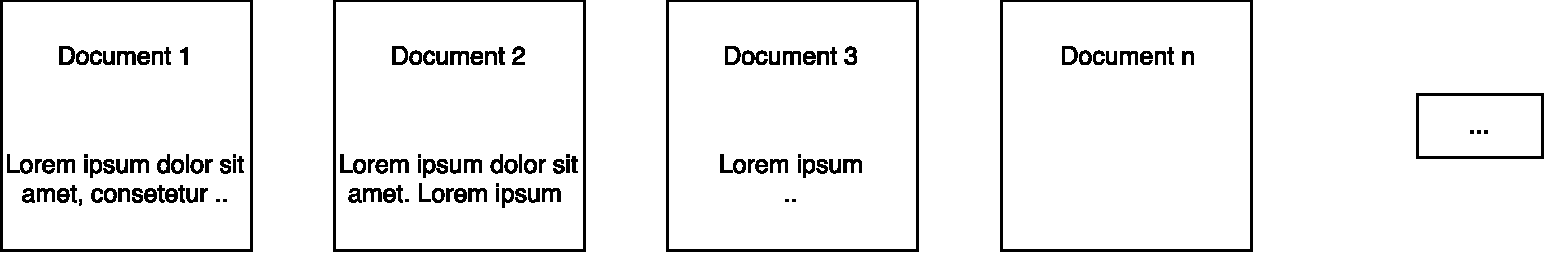
\includegraphics[scale=0.4]{pdf/Documents.pdf}\\
		\bigskip
		Zugriffszeit auf Festplatte als Bottelneck
	}	
	
	

	\section{Index Creation}
	\frame{\frametitle{Index Creation}
	geeignete Datenstruktur um Zugriff auf die Festplatte zu minimieren
	\bigskip
	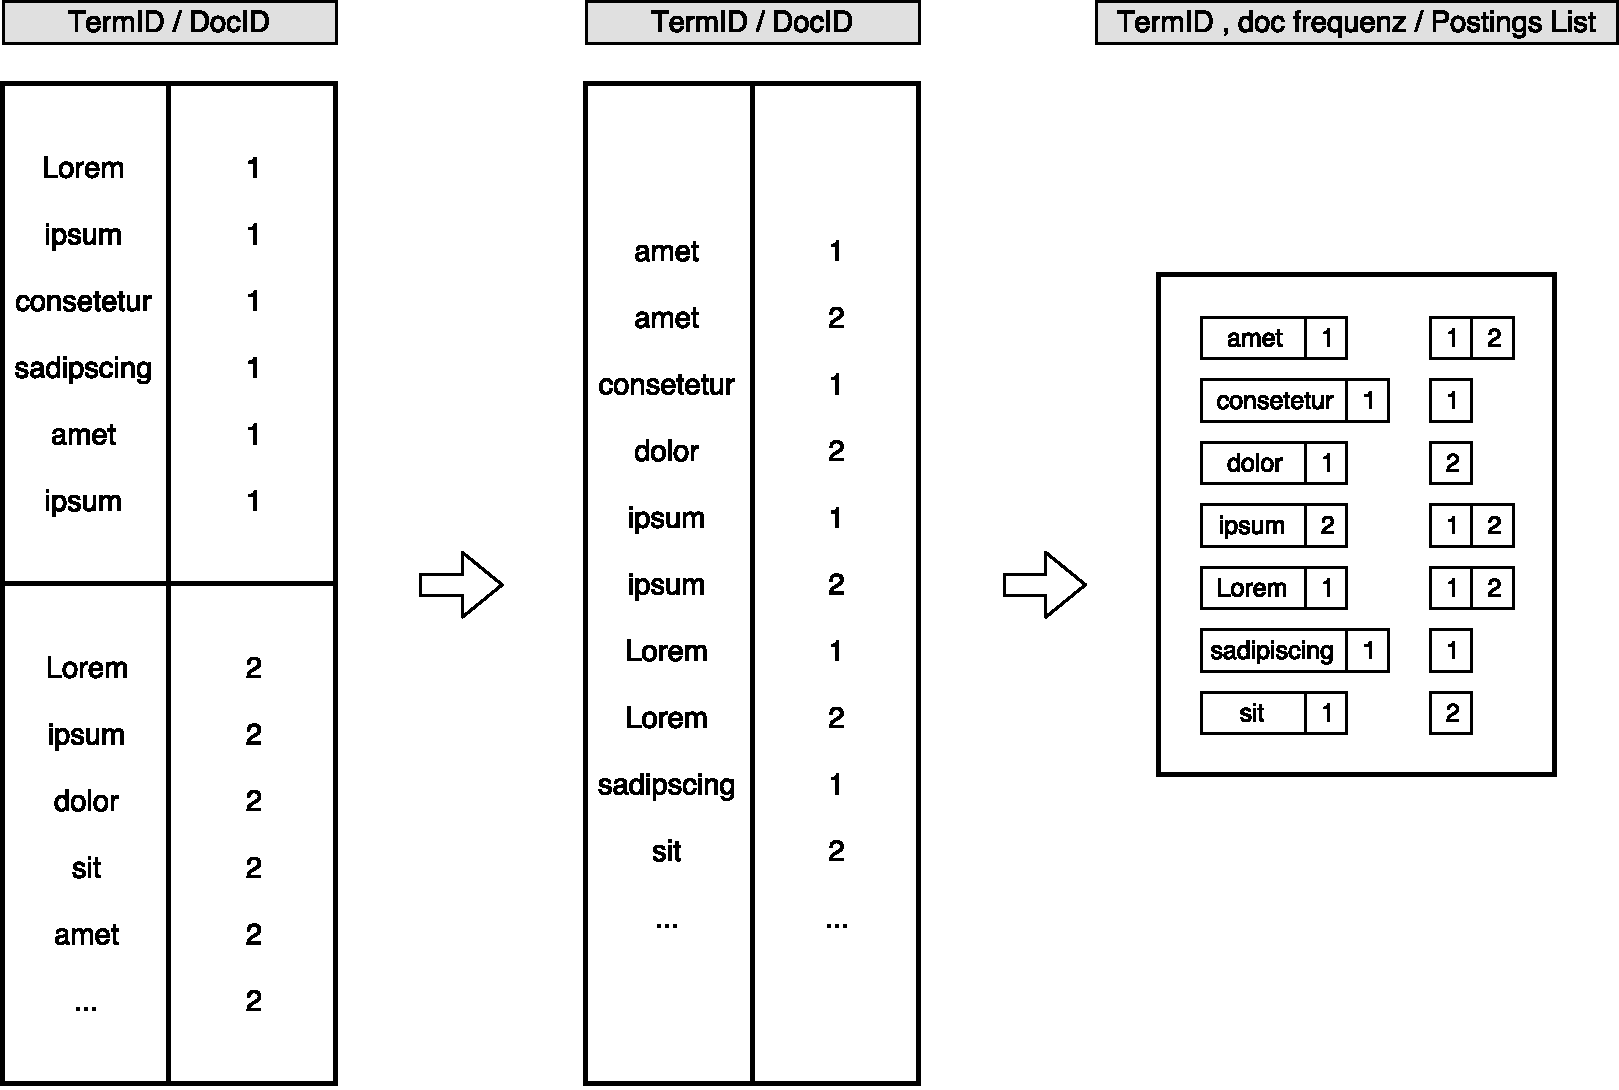
\includegraphics[scale=0.4]{pdf/PostingsList.pdf}

}

\subsection{Blocked sort-based indexing}
	 	\frame{\frametitle{Index Creation - hardware constraints}
		in der Regel übersteigt die Datenmenge der Dokumente den Main Memory.\\
		\bigskip
		\bigskip
		Reuters-RCV1 benötigt ca 0.8 GB für die termID/DocID Paare, bereits die DBLP übersteigt die Dokumentenanzahl, besitzt jedoch weniger Terme.
	}
	
		\frame{\frametitle{Blocked sort-based indexing (BSI)}
	todo: erklären usw
}
	
		\frame{\frametitle{Blocked sort-based indexing (BSI)}
\only<1>{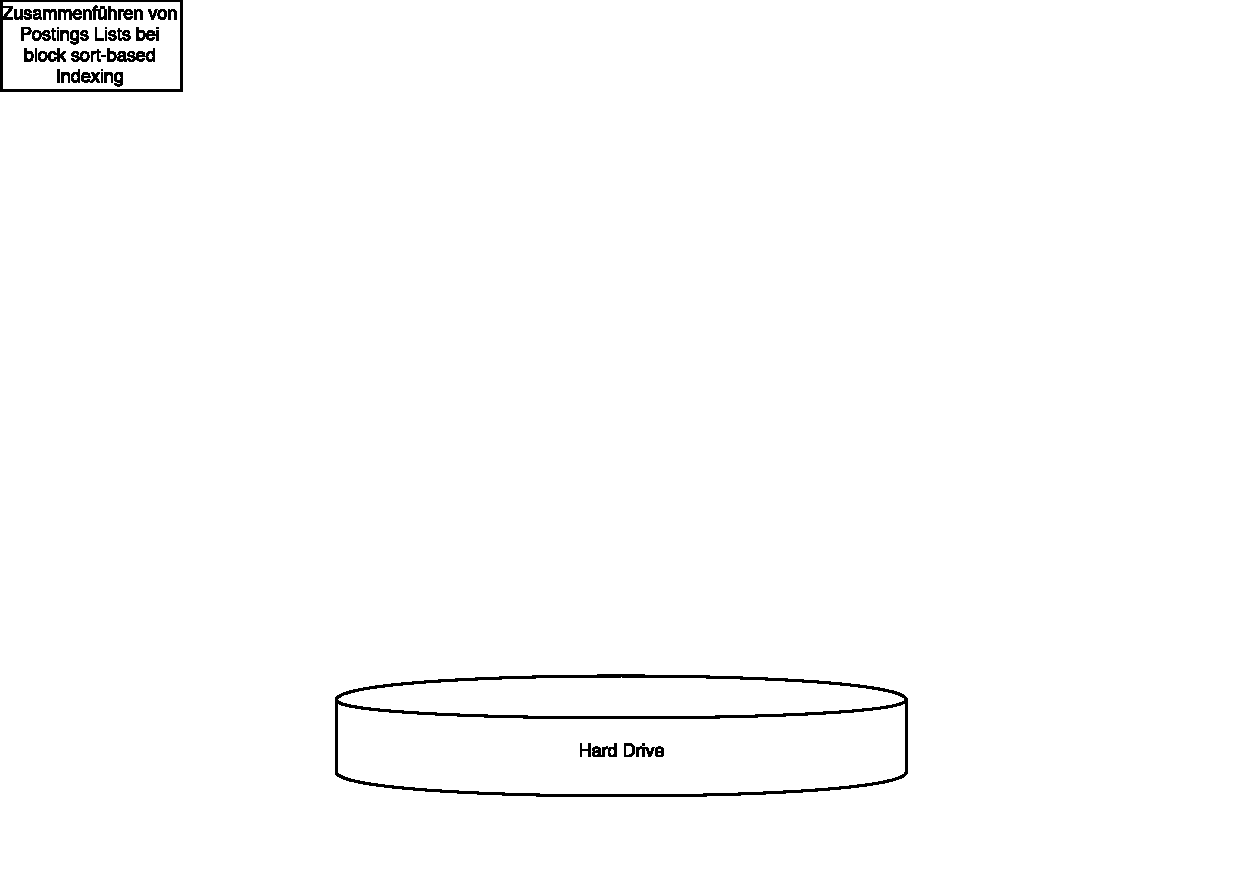
\includegraphics[scale=0.55]{pdf/BSI_merging1.pdf}}
\only<2>{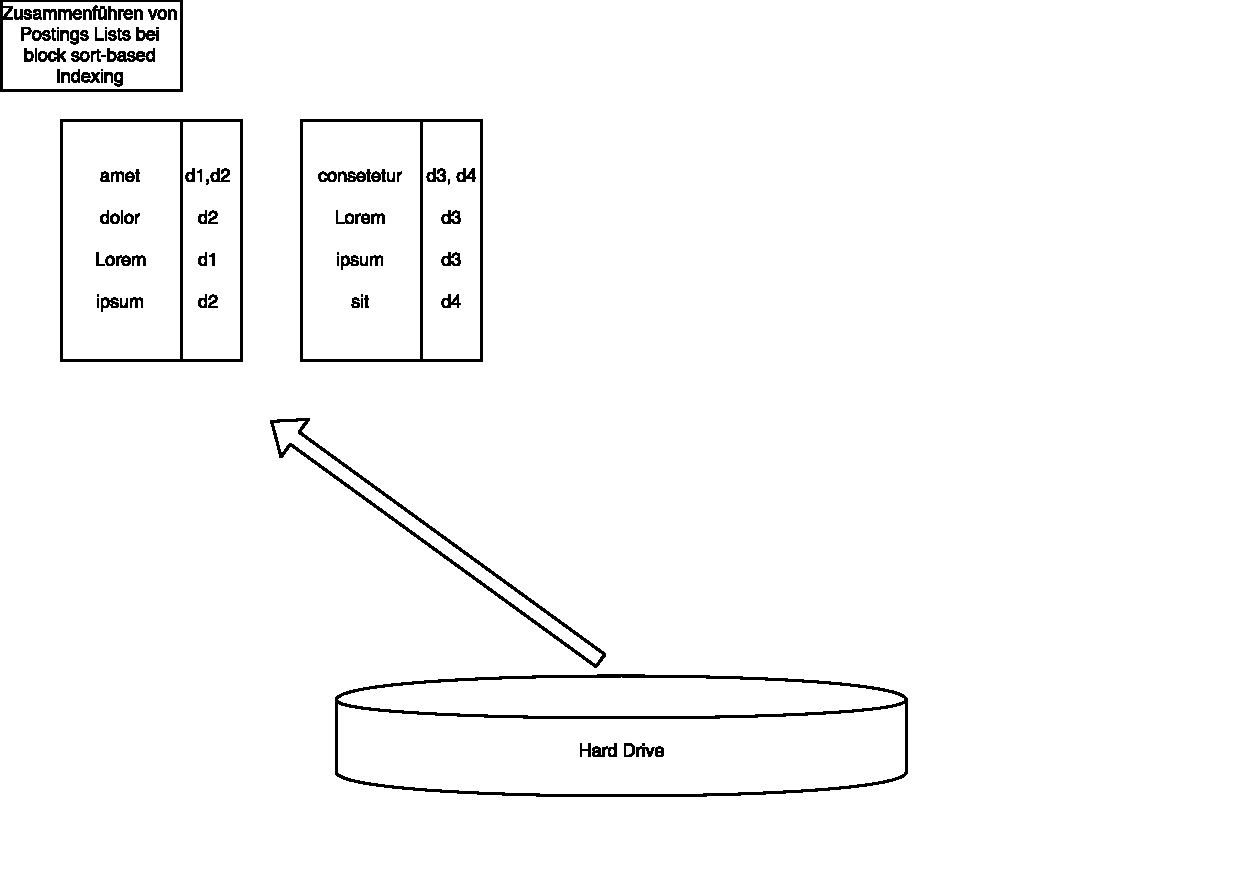
\includegraphics[scale=0.55]{pdf/BSI_merging2.pdf}}
\only<3>{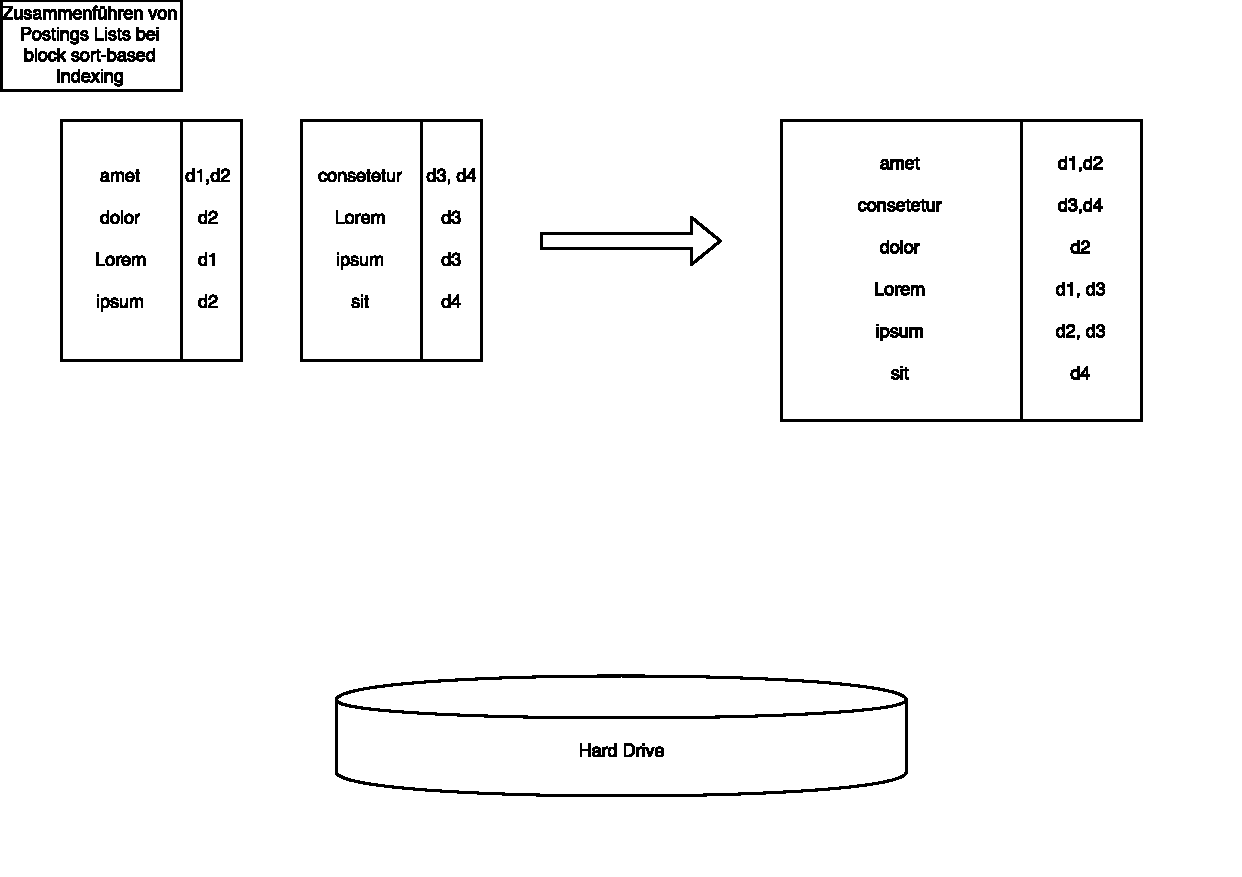
\includegraphics[scale=0.55]{pdf/BSI_merging3.pdf}}
\only<4>{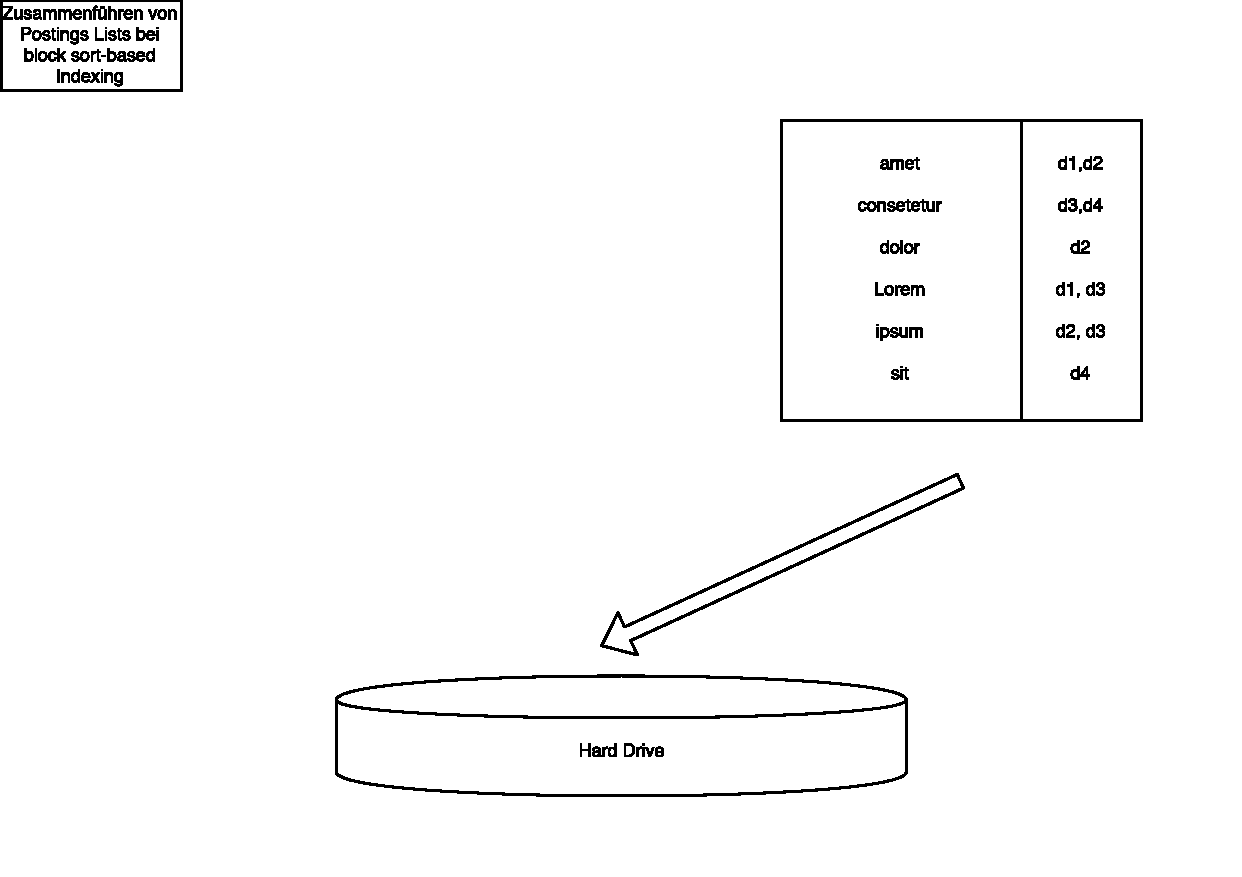
\includegraphics[scale=0.55]{pdf/BSI_merging4.pdf}}
}

	
\subsection{Single-pass in-memory indexing}
			\frame{\frametitle{Single-pass in-memory indexing (SPIMI)}
	
}

\subsection{Distributed indexing}
\subsection{Dynamic indexing}
\subsection{andere Indexverfahren}

\section{Fazit}

\section{Quellen}
	 	 \frame{\frametitle{Quellen}
	
	\begin{itemize}
		\item Shannon, C. E. \enquote{A Universal Turing Machine with Two Internal States.} Automata Studies. Princeton, NJ: Princeton University Press, pp. 157-165, 1956. \footnote{\url{http://www.sns.ias.edu/~tlusty/courses/InfoInBio/Papers/Shannon1956.pdf}}
		\item Wolfram Research and Wolfram, S. \enquote{The Wolfram 2,3 Turing Machine Research Prize.} \footnote{\url{http://www.wolframscience.com/prizes/tm23/}}
		\item Wolfram, S. A New Kind of Science. Champaign, IL: Wolfram Media, pp. 706-711 and 1119, 2002.
	\end{itemize}
	 
	 }
	
	
	
\end{document}
